\chapter{Development}
\label{chapter:dev}

On this chapter we will be explaining how the system was implemented, which algorithms that were used, the reason for choosing them, and what were the challenges faced during development.

The system was developed in the Unity Game Engine, utilizing the C\# language. The basis for this work was started by following the video tutorial available at \textcite{taft:2019}, about creating a 2D top-down game in Unity. This tutorial laid our foundation for important concepts, like importing the tileset, understanding how to draw a map, the basics of collision, etc.

It was after this point that the creation of the PCG system really started. To better understand its implementation, we will divide it in 7 steps and discuss each one in a different Section of this Chapter. The last Section will cover all of the user inputs that can be provided to the system in order to tune the map generation. However, first, there are still some information that are useful to understand all the steps from this point forward: 
\begin{itemize}
    \item The generated map will be represented by a global matrix of integers with width \(w_{map}\) and height \(h_{map}\).
    \begin{itemize}
        \item Its important to notice that \(w_{map}\) and \(h_{map}\) are user-defined parameters.
    \end{itemize}
    \item Each individual position of this matrix will be referred to as a \emph{cell}.
    \item A cell of value \(1\) represents a \emph{wall}, a cell of value \(0\) represents the absence of a \emph{wall}, or a path.
    \item The Figures where the map is shown are created by the use of Unity's Gizmo debugging tool. On these figures, the white color represents a \emph{path} cell and the black color represents a \emph{wall} cell.
    \item A group of one or more connected \emph{path} cells is here defined as a room.
\end{itemize}

\section{Create a randomly-filled base map}
\label{sec:randomf}

The first step taken was to have a randomly generated base map to start building upon. The generation of random or pseudo-random content is a part of most PCG techniques. In our case, the importance of the randomness is a reflection of one of the items for what is considered a good map, pointed on Section \ref{sec:goodmap}: "the Generated maps should look different from one another".

The creation of this base map is accomplished by the steps listed here in Algorithm \ref{alg:randomgen}.


\begin{algorithm}[h] 
 \DontPrintSemicolon
 int map[\(w_{map},h_{map}\)]\;
 \SetKwFunction{FillMapRandomly}{FillMapRandomly}
 \SetKwProg{Fn}{Function}{:}{}
 \Fn{\FillMapRandomly{}}{
  \For{all cells in the map}{
   random = randomly generated number between 0 and 100\;
   \eIf{random < fillPercent}{
    map cell = 1\;
   }{
    map cell = 0\;
   }
  }
 }
 \caption{Randomly filling of the map}\label{alg:randomgen}
\end{algorithm} 

The variable \(fillPercent\) specifies how much of the map will be populated by \emph{walls} or \emph{paths}, this variable is a user-defined parameter. The attribution of different values to it will generate different maps at the end of the process. Figure \ref{fig:fillper50} shows an example of a base map with \(w_{map} = h_{map} = 50\) and  \(fillPercent = 50\), while Figure \ref{fig:fillper80} shows the same map but with \(fillPercent = 80\).

\begin{figure}[h]
  \centering
  \begin{minipage}[b]{0.4\textwidth}
    \caption{Map with fillPercent = 50.}
    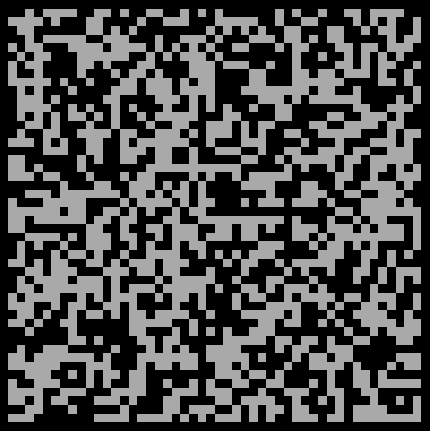
\includegraphics[width=\textwidth]{images/development/50_filled.png}
    \legend{Source: Image provided by author}
    \label{fig:fillper50}
  \end{minipage}
  \hfill
  \begin{minipage}[b]{0.4\textwidth}
    \caption{Map with fillPercent = 80.}
    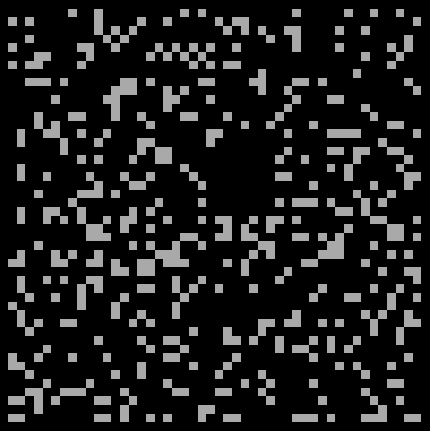
\includegraphics[width=\textwidth]{images/development/80_filled.png}
    \legend{Source: Image provided by author}
    \label{fig:fillper80}
  \end{minipage}
\end{figure}

The random number generator used to fill the map can also be controlled by a user-defined parameter. The user can choose to write a \emph{seed} for the generator, which is a text that will tune the generator. Different executions of the generator with the same \emph{seed} will always give the same results. In this case the generated map will always be the same for each given \emph{seed}. Otherwise, the \emph{seed} will be automatically chosen based on the execution time of the algorithm, making each generation different from the previous ones.

\section{Cellular automata}

A CA is a discrete model of computation that was first discovered by Stanislaw Ulam and John von Neumann; it can be described, in a simplified manner, as an \(n\)-dimmensional grid, with a set of states and a set of transition rules. The grid is composed by cells, each of them able to be in one of several states; in its most basic form, cells can be 1 (on) or 0 (off) \cite{wolfram:1983}.

Although CA has found application in many different areas of study, it was the 1970s Conway's Game of Life which brought its attention to beyond academia. This was a zero-person game where cells from a 2D grid would live or die (hence, they had only two states, \(1\) or \(0\)) based on how many neighbors they had around them. This neighborhood is defined as the eight (8) cells surrounding the central cell currently being analyzed. Some of the rules from the Game of Life have been applied in dungeon generation because of the cave-like appearance that the algorithm creates on the grid \cite{shaker:2016}.

In our specific case, the rule used is that, if there are more than \(4\) \emph{walls} around the current cell, then the cell becomes a \emph{wall}, if there are less than \(4\) \emph{walls} around the cell, it becomes a \emph{path}. The method was also chosen because it generates images that are similar to the representation of \emph{spongework} caves, shown in Figure \ref{fig:cave_patterns}. Figure \ref{fig:ca_rule} serves as a visual representation to this rule, where the red cell is the one under current analysis, while the number on the right represents is resulting state after the CA execution.

\begin{figure}[h]
    \caption{Representation of the CA rule used.}
    \centerline{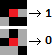
\includegraphics[width=4cm]{images/development/ca_rule.png}}
    \legend{Source: Image provided by author}
    \label{fig:ca_rule}
\end{figure}

In Figure \ref{fig:5itca} we can see the base map generated in Figure \ref{fig:fillper50} after \(5\) iterations of the CA. In addition, Figure \ref{fig:20itca} shows the map after \(20\) iterations. The number of iterations is a user-defined parameter for the system.

\begin{figure}[h]
  \centering
  \begin{minipage}[b]{0.4\textwidth}
    \caption{Map after 5 iterations of CA.}
    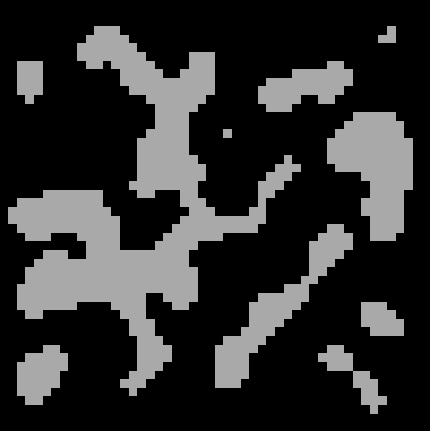
\includegraphics[width=\textwidth]{images/development/5it_ca.png}
    \legend{Source: Image provided by author}
    \label{fig:5itca}
  \end{minipage}
  \hfill
  \begin{minipage}[b]{0.4\textwidth}
    \caption{Map after 20 iterations of CA.}
    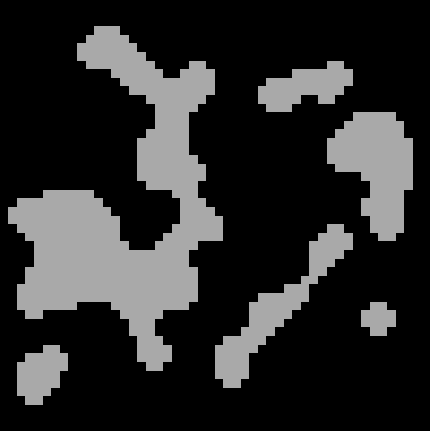
\includegraphics[width=\textwidth]{images/development/20it_ca.png}
    \legend{Source: Image provided by author}
    \label{fig:20itca}
  \end{minipage}
\end{figure}

\section{Creating a list of rooms}

At this stage, the algorithm has finished letting us with one or more rooms scattered throughout the map. On code, we represent the rooms as a separate \emph{Room} class that contains the coordinates of all of its cells. It is important to note that the \emph{Room} class also contains other important information used by a following step of the algorithm (Section \ref{sec:connection}) defined by a flag indicating if the \emph{Room} was visited, a list of \emph{Rooms} connected to this \emph{Room} and a method that connects two \emph{Rooms}.

There are two sets of user-defined inputs that will determine if there will be the creation of entrance and exit rooms and their location on the map. After that is completed, the algorithm goes through the map grid and searches for \emph{paths}. If a \emph{path} was found we use the flood-fill algorithm in order to define where this room begins and where it ends, and then, we create a \emph{Room} containing all the coordinates of its cells. After the creation of the \emph{Room} it is added to a list containing all \emph{Rooms} on the map.

\section{Checking if the generated map is possible}
\label{sec:check_poss}

One of the issues that came up during development is that not all generated maps can translate well to a 2D top-down tile-based map. This happens because, for a visually well-formed wall to be generated, there needs to have at least \(2\) \emph{walls} between \(2\) \emph{paths}. On that respect, Figure \ref{fig:malformed_wall} exemplifies a malformed wall between 2 \emph{Rooms}.

\begin{figure}[h]
    \caption{Example of a malformed wall between two \emph{Rooms}}
    \centerline{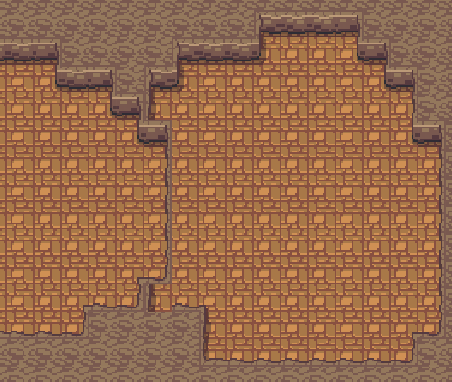
\includegraphics[width=10cm]{images/development/deformed_wall.png}}
    \legend{Source: Image provided by author}
    \label{fig:malformed_wall}
\end{figure}

To solve this matter, in this step we go through each cell of each \emph{Room} and check if there are \emph{Rooms} that have a distance of less than \(2\) cells from each other. If there are, then the whole process is started again until the generated \emph{Room} can be well translated to a tile-based map. Algorithm \ref{alg:check_possible} describes this process.

\begin{algorithm}[h]
 \DontPrintSemicolon
 \While{map is not possible}{
  Randomly fill the map\;
  Run cellular automata\;
  Create a list of Rooms\;
  Check if the generated map is possible\;
 }
 \caption{Checking if the generated map is possible}
\label{alg:check_possible}
\end{algorithm} 

\section{Connection between rooms}
\label{sec:connection}

To better explain how we create connections between separated rooms we will divide this section in two: ensuring connectivity through graph algorithms and drawing the connection between rooms using Bresenham's line algorithm.

\subsection{Ensuring connectivity}

Ensuring the connectivity between all rooms is important for, as mentioned on Section \ref{sec:goodmap}: "Dungeon maps should have a point of entrance, a point of exit (which might be the same as the point of entrance) and a path between them". For our specific case, there is one more reason why this step is important: making maps that are similar to the \emph{branchwork} or \emph{network} cave patterns previously seen on Figure \ref{fig:cave_patterns}.

As the guideline above recalls, we need to make sure that every pair of \emph{Rooms} are connected, i.e., there is a way to reach one \emph{Room} by starting on any other \emph{Room}. Each \emph{Room} in the map can be viewed as a node in a graph, that way, we made use of a popular algorithm in graph theory to check if there's connectivity: Depth-First Search (DFS). DFS is an algorithm that starts at an arbitrary node of the graph and explores as far as possible along each branch before backtracking \cite{even:2011}.

Figure \ref{fig:connectivity} shows a visual representation of the algorithm used in this step, which is described in Algorithm  \ref{alg:connectivity}. Each node of the graph represents a \emph{Room} in the map. In quadrant \(1\) we start with a map with fully disconnected \emph{Rooms}. Then, the algorithm begins by connecting each node to its closest node, as seen in quadrant \(2\); following that, it performs the DFS to check if connectivity is ensured; if not, it handles the sets of connected nodes a a single node, like is shown on quadrant \(3\), and then, redo the connectivity step, which leads to the result that can be seen in quadrant \(4\).

\begin{figure}[h]
    \caption{Visual representation of the connectivity algorithm.}
    \centerline{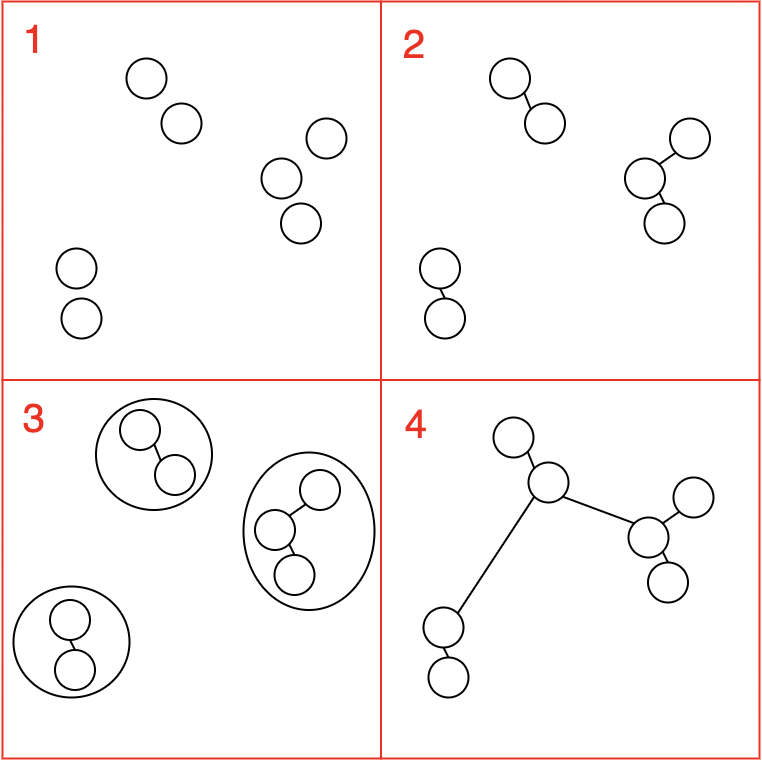
\includegraphics[width=7cm]{images/development/graph_connect.png}}
    \legend{Source: Image provided by author}
    \label{fig:connectivity}
\end{figure}

\begin{algorithm}[h]
 \DontPrintSemicolon
 Graph = represent Rooms as graph\;
 \While{connectivity isn't reached}{
  Connect closest Rooms in Graph\;
  Check connectivity\;
  Transform the sets of connected Rooms into new nodes for the new Graph\;
 }
 \caption{Ensuring connectivity of the map}
\label{alg:connectivity}
\end{algorithm} 

\subsection{Drawing the connection}

At this point of the algorithm, we have a map filled with \emph{Rooms} that have ensured connectivity, nonetheless, this connectivity is only represented by some elements of the \emph{Room} class, being not represented yet in the map grid as \emph{walls} and \emph{paths}.

This is where the algorithm known as Bresenham's line is used. This algorithm, suggested in 1962 by Jack Elton Bresenham, is used to determine which points on an \(n\)-dimensional raster should be selected in order to form a close approximation of a straight line \cite{bresenham:1965}. 

Since each \emph{Room} has all of its cell coordinates stored, we can choose the closest cells for each connection and then use the Bresenham's line algorithm to draw this straight line on the map. Figure \ref{fig:map_connected} shows the same map seen in Figure \ref{fig:20itca} after the connectivity is ensured and then drawn on the map using Bresenham's algorithm.

On a first glance, it may seem like these passages will not be wide enough to allow the player to pass through them, but the nature of the chosen tileset ensures that this is indeed possible, as shown in Figure \ref{fig:it_works}.

\begin{figure}[h]
    \caption{Map after connectivity is ensured.}
    \centerline{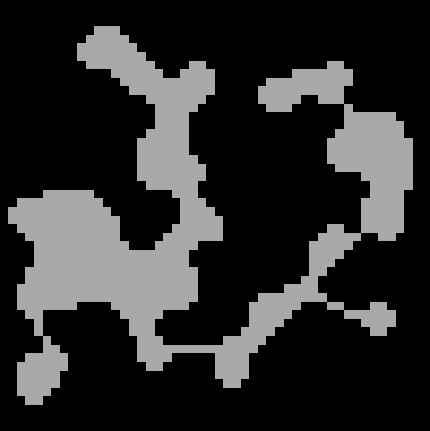
\includegraphics[width=7cm]{images/development/after_connection.png}}
    \legend{Source: Image provided by author}
    \label{fig:map_connected}
\end{figure}

\begin{figure}[h]
    \caption{Passage before and after tile placement.}
    \centerline{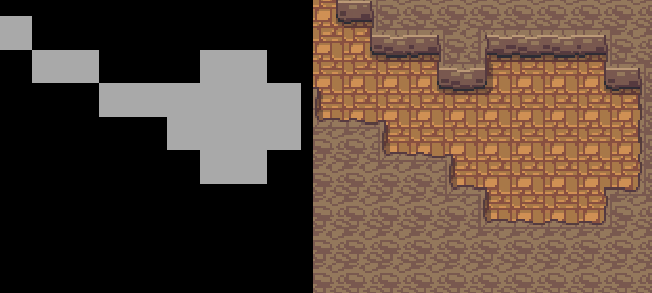
\includegraphics[width=7cm]{images/development/it_works.png}}
    \legend{Source: Image provided by author}
    \label{fig:it_works}
\end{figure}

\section{Removing inconsistencies from the map}

Just like in Section \ref{sec:check_poss}, maps that are generated with single-spaced \emph{walls} will not translate well to a 2D tile-map. Some of these problematic \emph{walls} are occasionally created on the process of drawing the Bresenham's lines to connect separate \emph{Rooms}.

In this step we deal with these \emph{inconsistencies} by going through the entire map grid and checking for \emph{wall} cells that have either a \emph{path} to its right and left, here shown on Figure \ref{fig:hor_inc}; or to its up or down, as shown in Figure \ref{fig:ver_inc}; the inconsistencies are circled in red. After these inconsistent single-spaced \emph{walls} are found, they are replaced by \emph{paths}.

\begin{figure}[h]
  \centering
  \begin{minipage}[b]{0.4\textwidth}
    \caption{Example of a horizontal inconsistency.}
    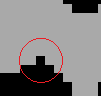
\includegraphics[width=\textwidth]{images/development/horizontal_incosistency.png}
    \legend{Source: Image provided by author}
    \label{fig:hor_inc}
  \end{minipage}
  \hfill
  \begin{minipage}[b]{0.4\textwidth}
    \caption{Example of a vertical inconsistency.}
    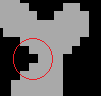
\includegraphics[width=\textwidth]{images/development/vertical_incosistency.png}
    \legend{Source: Image provided by author}
    \label{fig:ver_inc}
  \end{minipage}
\end{figure}

\section{Tile placement}

Finally, the last step of the generation is to place the tiles to their corresponding spots in the \emph{walls} and \emph{paths}. There are a number of \(13\) \emph{wall} tiles needed to create the map, which are shown here on Figure \ref{fig:wall_tiles}. There is only a single tile that corresponds to a \emph{path}, which is visible on the resulted map in Figure \ref{fig:map_result}.

\begin{figure}[h]
    \caption{Wall tiles.}
    \centerline{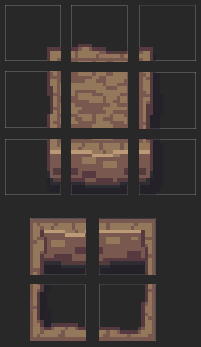
\includegraphics{images/development/wall_tiles.png}}
    \legend{Source: Image provided by author}
    \label{fig:wall_tiles}
\end{figure}

The first idea we had was to try to use a custom CA ruleset, where each cell had \(14\) possible states, one for each needed tile. However, after we assessed that a single execution of the ruleset through the map grid was enough to place all the tiles correctly, it was our understading that our algorithm could be better described as a morphological operation.

This morphological operation, containing 14 rules, is here shown on Figure \ref{fig:ruleset}. The next item list serves to better understand the content of this Figure:

\begin{itemize}
    \item Similar to Figure \ref{fig:ca_rule}, the center cell is the one currently being analyzed.
    \item Gray cells represent \emph{wall} cells.
    \item White cells represent \emph{path} cells.
    \item Pink cells represent either a \emph{wall} or a \emph{path}, meaning that the content of this cell is not taken into account, i.e., it won't be analyzed by this rule.
    \item The tile next to the rule number is what the rule will return for the cell being analyzed. 
\end{itemize}

For example, \emph{Rule 3} will check if the current cell, the one at the center of the grid, is a \emph{wall}, then if the cell above it is a \emph{path}, then if the cell to the left of it is a \emph{path}, then if the cell to the right of it is a \emph{wall}, then if the cell below it is a \emph{wall} and finally if the cell to the bottom right of it is a \emph{wall}; if all of these conditions are met, the rule will return the corner tile shown on Figure \ref{fig:ruleset} for \emph{Rule 3} and place it on the analyzed cell.

\begin{figure}[h]
    \caption{Ruleset.}
    \centerline{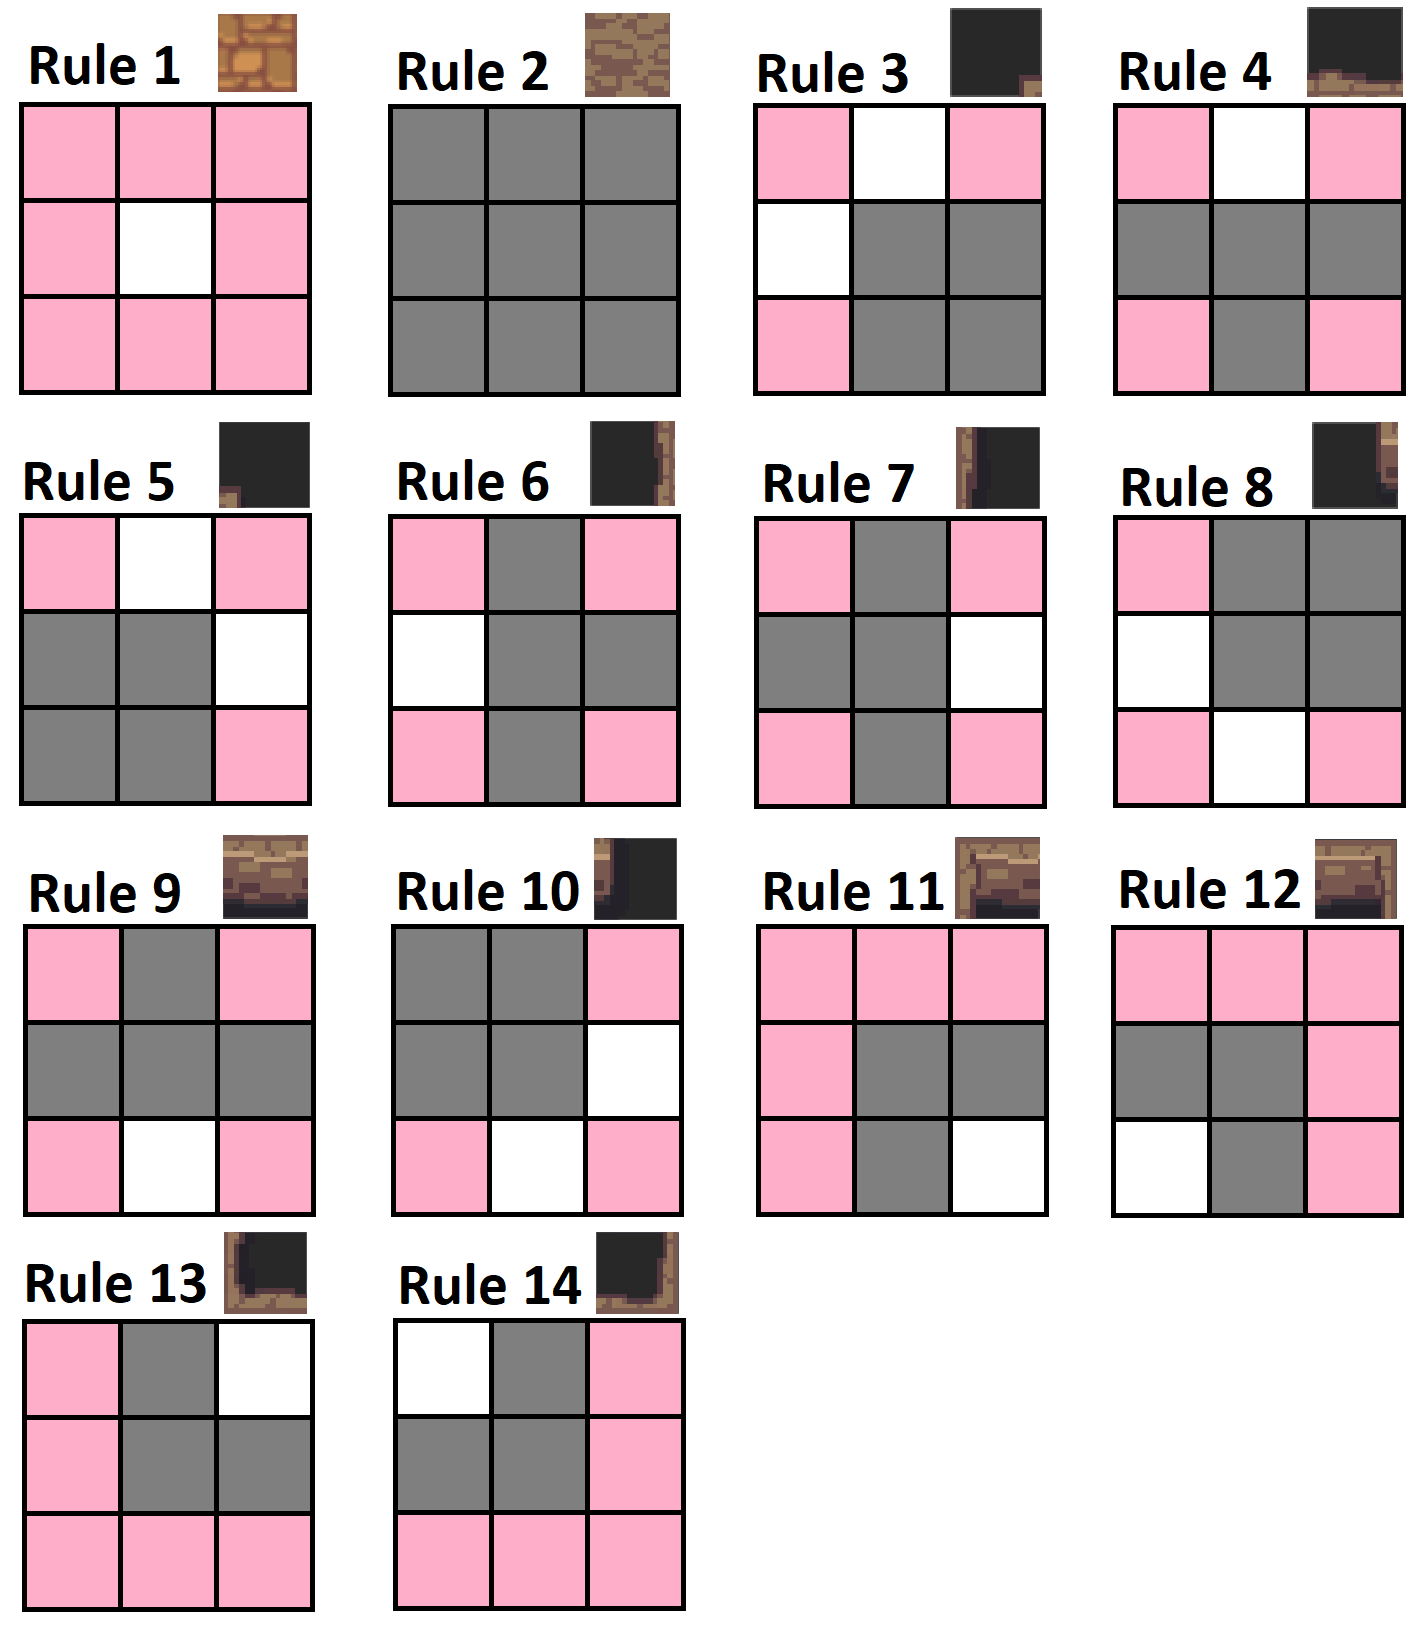
\includegraphics[width=12cm]{images/development/morph_rules.png}}
    \legend{Source: Image provided by author}
    \label{fig:ruleset}
\end{figure}

After the algorithm has gone through the whole map grid, the result will be a fully-formed 2D tile-based top-down map. Figure \ref{fig:map_result} shows the same map from Figure \ref{fig:map_connected} after the tile placement.

\begin{figure}[h]
    \caption{Resulting generated map.}
    \centerline{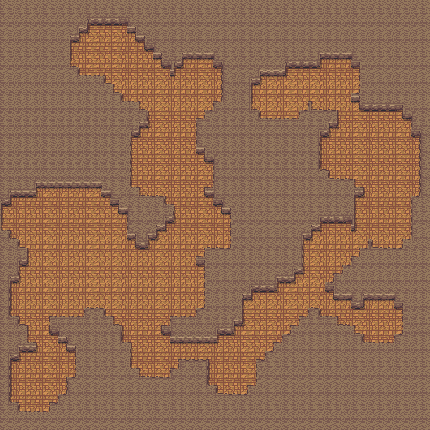
\includegraphics{images/development/final_result.png}}
    \legend{Source: Image provided by author}
    \label{fig:map_result}
\end{figure}

\section{User-defined parameters}

On this section we will be showcasing all of the user-defined parameters that can be used to tune the generation of the map.

Figure \ref{fig:user_par} shows a snippet of the Unity tool, showing all the parameters used to generate the map that was seen on Figure \ref{fig:map_result}: \(w_{map} = h_{map} = 50\); the creation of a start and an end room was disabled, meaning that the cave used as an example was created without entrance and exit; the number of iterations for the CA step was set to \(20\); a specific \emph{seed} was set; and the fill percent of the first step was set to \(50\).

The parameters can be explained as such:
\begin{itemize}
    \item \textbf{Width}: the number of cells on a row of the generated map, or \(w_{map}\).
    \item \textbf{Height}: the number of cells on a column of the generated map, or \(h_{map}\).
    \item \textbf{Create Start/End Room}: toggles the creation of an entrance/exit for the generated cave map.
    \item \textbf{Start/End X/Y 1/2}: the coordinates of the 2 cells that will compose the entrance/exit of the cave map.
    \item \textbf{Iterations}: number of times that the CA algorithm will execute on the map.
    \item \textbf{Seed}: a text that will tune the random number generator, can be set to always generate the same map.
    \item \textbf{Use Random Seed}: this will define if the Seed from the above parameter will be used or if the system will choose a random one.
    \item \textbf{Random Fill Percent}: define the value of the variable \(fillPercent\), explained on Section \ref{sec:randomf}. 
\end{itemize}

\begin{figure}[h]
    \caption{Available user parameters.}
    \centerline{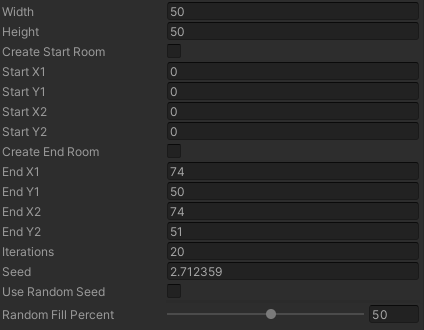
\includegraphics{images/development/user_parameters.png}}
    \legend{Source: Image provided by author}
    \label{fig:user_par}
\end{figure}